
\subsection*{Hint for Review Problem~\ref{UandV}}

{\ttfamily
\fontdimen2\font=0.4em
\fontdimen3\font=0.2em
\fontdimen4\font=0.1em
\fontdimen7\font=0.1em
\hyphenchar\font=`\-

\hypertarget{subspaces_and_spanning_sets_hint}{For} the first part, try drawing an example in ${\mathbb R}^3$:
\begin{center}
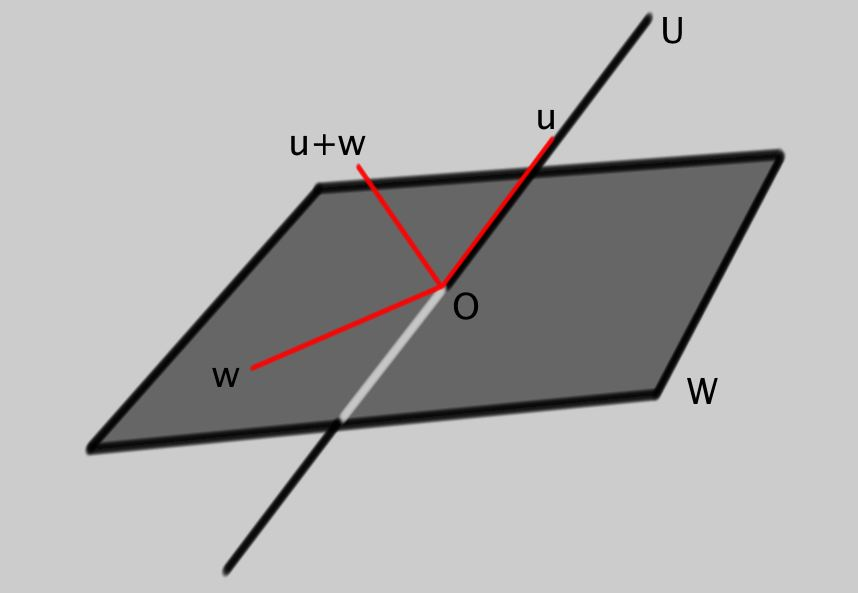
\includegraphics[scale=.35]{UunionW.jpg}
\end{center}
Here we have taken the subspace $W$ to be a plane through the origin and
$U$ to be a line through the origin. The hint now is to think about what happens when 
you add a vector $u\in U$ to a vector $w\in W$. Does this live in the union $U\cup W$?

For the second part, we take a more theoretical approach. Lets suppose that $v\in U\cap W$ and $v'\in U\cap W$. This implies
$$
v\in U \quad \mbox{and} \quad v'\in U\, .
$$
So, since $U$ is a subspace and all subspaces are vector spaces, we know that the linear
combination
$$
\alpha v+\beta v'\in U\, .
$$
Now repeat the same logic for $W$ and you will be nearly done.


} % Closing brace for the font

%\newpage
